\documentclass{beamer}
\usetheme{Boadilla}
\title{Decide Doctoral School}
\subtitle{Introduction and Research outlines}
\author{M. Rahmani}
\institute{University of Klagenfurt}
\date{\today}
\begin{document}
	\begin{frame}
		\titlepage
	\end{frame}
	\begin{frame}
		\frametitle{Who am I?}		
		\begin{itemize}
			\item \textbf{Name}: Mohammad Rahmani
			\item \textbf{Education}:
				\begin{itemize}
					\item \textbf{Bachelor}: Applied Mathematics, Shiraz University
					\item \textbf{Masters}: Computer science (Expert systems), Tehran Polytechnic
				\end{itemize}
		\end{itemize}		
	\end{frame}
	
	\begin{frame}
		\frametitle{Who am I? Previous experience}		
		Professional experience in
		\begin{itemize}
			\item Data science
			\item Computer vision
			\item Deep learning
			\item Reinforcement learning
			\item statistical inference
		\end{itemize}		
	\end{frame}
	
	\begin{frame}
		\frametitle{Decision making in Self-aware Single Robot Systems}
		\begin{itemize}
			\item \textbf{Self-awareness definition}: The capacity that an Intelligent Agent becomes the object of its own attention that is:
				\begin{itemize}
					\item Contextually placing externally and internally perceived data together by a robot and deduct learning models out of it.
				\end{itemize}   
		\end{itemize}		
	\end{frame}

	\begin{frame}
		\frametitle{Example Single Robot Systems}
		\begin{itemize}
				\item Sample training data $v_{t_1}=100kmph$ , $s_{35^{\circ}-20m}$ , $v_{t_2}=60kmph$ (Here the model should learn to increase speed by 40kmph after such a slope)
		\end{itemize}
		\begin{figure}
			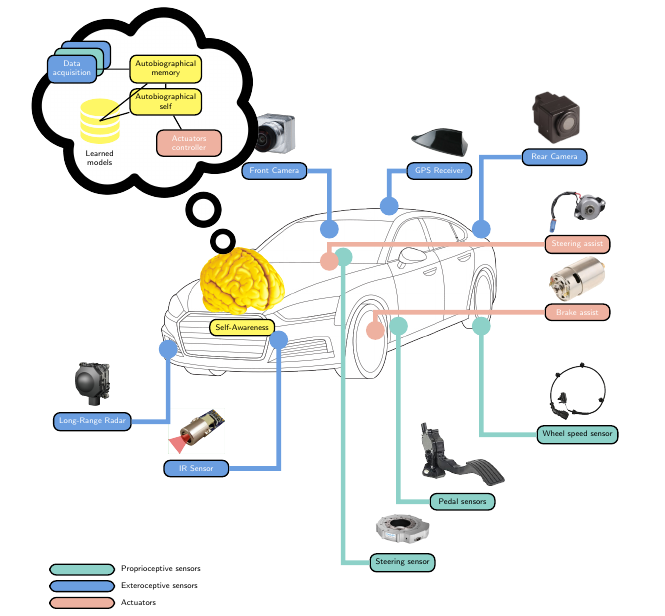
\includegraphics[scale=0.3]{regazzoni-2020-multi-sensorial-generative-and-descriptive-self-awareness-models-for-autonomous-systems-fig-1.png}
			\caption{Ref: Regazzoni, Marcenaro, Campo, Rinner. Multi-sensorial generative and descriptive self-awareness models for autonomous systems. 2020 IEEE}
		\end{figure}		
	\end{frame}

	\begin{frame}
		\frametitle{Decision making notion in self-aware systems}
		\begin{itemize}
			\item \textbf{Decision making in SA systems}: refers to the ability to generate signals that can be employed by the agent’s control system such that its actions are self-monitored dynamically.
			\item \textbf{Topical literature}: 
				\begin{itemize}
					\item Lewis, Platzner, Rinner, Torresen. Self-aware Computing systems, an engineering approach. 2016. Springer
					\item Kounev, Kephart, Milenkoski, Zhu. Self-aware Computing systems. Springer
					\item The Proceedings of IEEE on Self-Awareness for Autonomous Systems in July 2020
				\end{itemize}
		\end{itemize}	
	\end{frame}

	\begin{frame}
		\frametitle{What we plan to do?}
		Extending self-aware decision making to MRS:
		\begin{itemize}
			\item Global system state information to control it's decisions has a natural, distributive nature.
			\item \textbf{But} the system can \textbf{collectively} use this information to have a \textbf{sense} of the best \textbf{state} it should take in \textbf{future}.
		\end{itemize}	
	\end{frame}
	\begin{frame}
		\frametitle{Examples}
			\begin{itemize}
				\item \textbf{In nature}: Bee and ant colonies. The human immune system 
				\item \textbf{In robotics}: The COCORO project in which a group of robots with simple behavioral rules and local interactions may achieve collective awareness of a global state, distributed across the individual units.
				\item \textbf{URL}: http://zool33.uni-graz.at/artlife/cocoro
			\end{itemize}	
	\end{frame}
	\begin{frame}
		\frametitle{Even simpler example, our probable start point}
		\begin{itemize}
			\item A follower vehicle learns 4 times a trajectory from a leader vehicle by generating models from its speed and steering angle data it receives.
			\item A pedestrian comes across the normal trajectory. The leading vehicle's camera detects him and stops. The follower detects anomaly in the flow of speed/steering data and stops as well.  
		\end{itemize}
		\begin{figure}
			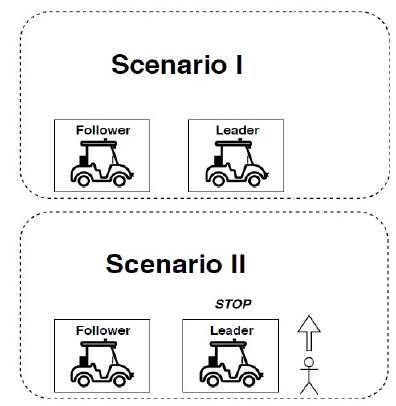
\includegraphics[scale=0.35]{two-icabs.png}
			\caption{Ref: Kanapram, Patrone, Plaza, Marchese, Bodanese, Marcenaro, Gomez, Regazzoni. Collective Awareness for Abnormality Detection in Connected Autonomous Vehicles, 2020, IEEE}
			\label{simple-collective-intelligence}
		\end{figure}	
	\end{frame}
\end{document}